\chapter{Name of Appendix}

\begin{itemize}
    \item AI model parameters
    \item Demo video
    \item Nav2 and Gazebo plugins
    \item domain.pddl, problem.pddl used in example
    \item Test sets and test results
    \item Mistral test model params
\end{itemize}

\section{Whisper experiments}
\subsection{Example test set}
The former FTX cryptocurrency mogul Sam Bankman-Fried was sentenced to 25 years in prison today for what prosecutors said was one of the biggest financial crimes in US history. A judge handed down that sentence after a jury this fall found Bankman-Fried guilty of seven different counts relating to fraud and money laundering. Bankman-Fried was found to have stolen at least \$8 billion from FTX customers. He was also ordered to pay \$11 billion today. Bankman-Fried has said he will appeal. For a closer look at this case, we’re joined by David Yaffe-Bellany. He’s covered this saga for years for The New York Times. David, thank you so much for being here. You were in the courtroom today when that sentence was handed down. I wonder what stood out to you the most from the judge’s sentence? I think what I was struck by the most was some of the language that the judge used to justify the length of the sentence. He didn’t just say these were really serious crimes. He said that Sam Bankman-Fried had to go to prison for 25 years because if he was let out any earlier, he might commit more crimes. Basically, there’s this sense that he hasn’t really expressed remorse for what happened and were he to get out, he might pitch a new company and try to commit a similar fraud to the one that brought down FTX. Is this because all along Bankman-Fried really hasn’t expressed a great deal of remorse about this, which I know judges love to see? Yeah. I mean, it’s complicated. He’ll say that he’s sorry about what happened and that he’s apologized to customers, he’s apologized to employees of FTX. But he obviously challenged the charges against him. He’s planning to appeal. So he hasn’t apologized for committing crimes because it remains his position that he hasn’t committed any crimes, but that certainly hurt him at the sentencing stage. For people who have not been following this as closely as you have, can you just remind us of the basic sort of flow of what happened here? How did FTX come crumbling down? Sure. So just 18 months ago, Sam Bankman-Fried was a huge star in the business world. He ran a cryptocurrency exchange, FTX, which was basically a platform where you could take your dollars and spend them to buy Bitcoin or Ether or other cryptocurrencies. And you could also store your crypto on the platform, so it kind of operated as a bank as well. It became really popular as the crypto industry grew and grew. And then in November 2022, there was essentially a run on the bank, and that exposed a big \$8 billion dollar hole in the money that FTX was supposed to be holding on behalf of its customers. And that kickstarted the series of events that brought the whole edifice crashing down. And so those people who had “banked” their money in his exchanges, they lost all the money. Those are the victims in this case? Those are one subset of the victims. They’re probably the largest subset. But the other victims include venture capital investors who put in more than a billion dollars into FTX, and also lenders who gave money to companies in Bankman-Fried’s empire. So the \$11 billion that he’s been ordered to pay, where is that supposed to go? That’s actually going to the US government. That’s not restitution that’s going to victims. But really, that number is kind of academic because Bankman-Fried does not have \$11 billion sitting around that he can just disperse to people. And really, the root for recoveries for the customers of FTX is through the bankruptcy process. So you’ve got a team of lawyers that took over the exchange after it collapsed and have spent the last almost year and a half cobbling together assets wherever they can find them to try to create a pool of funds that can be returned to the people who lost their money. But so far, those people have not yet been made whole. But that is the hope and/or expectation? That’s the hope, and the bankruptcy lawyers have said they’re expecting to make customers whole, but what being made whole means is complicated. They will receive the dollar value of their holdings on the FTX platform as of November 2022 when the bankruptcy happened. So that doesn’t account for the rapid surge in cryptocurrency prices over that period. So if you had one Bitcoin on FTX and it was worth \$20,000 in November, you’ll get \$20,000 back even though that Bitcoin would be worth \$70,000 today. I see. Many people have seen this case as an overarching stain on cryptocurrency writ large. And I wonder, do you think that that’s fair and is that actually what is happening? Does this say anything about cryptocurrency itself or is this just about one person’s potential crime here? I think there are specific characteristics of the crypto industry that helped enable this fraud. One sort of mechanism that Bankman-Fried was using to cover up some of his crimes was that he was inventing new currencies, new digital currencies, and then putting them up as collateral to borrow actual money from lenders. And so that’s a unique aspect of this kind of strange world of digital money that helped enable the fraud. I think it’s also the case that the crypto world has attracted a type of person who’s sort of inclined toward gambling, who wants to take lots of risks, and that says a lot about the culture of the industry and it’s part of what laid the foundation for this massive disaster. All right. David Yaffe-Bellany of The New York Times, thank you so much. Thanks for having me.

\subsection{Test result figures}

\begin{figure}
    \centering
    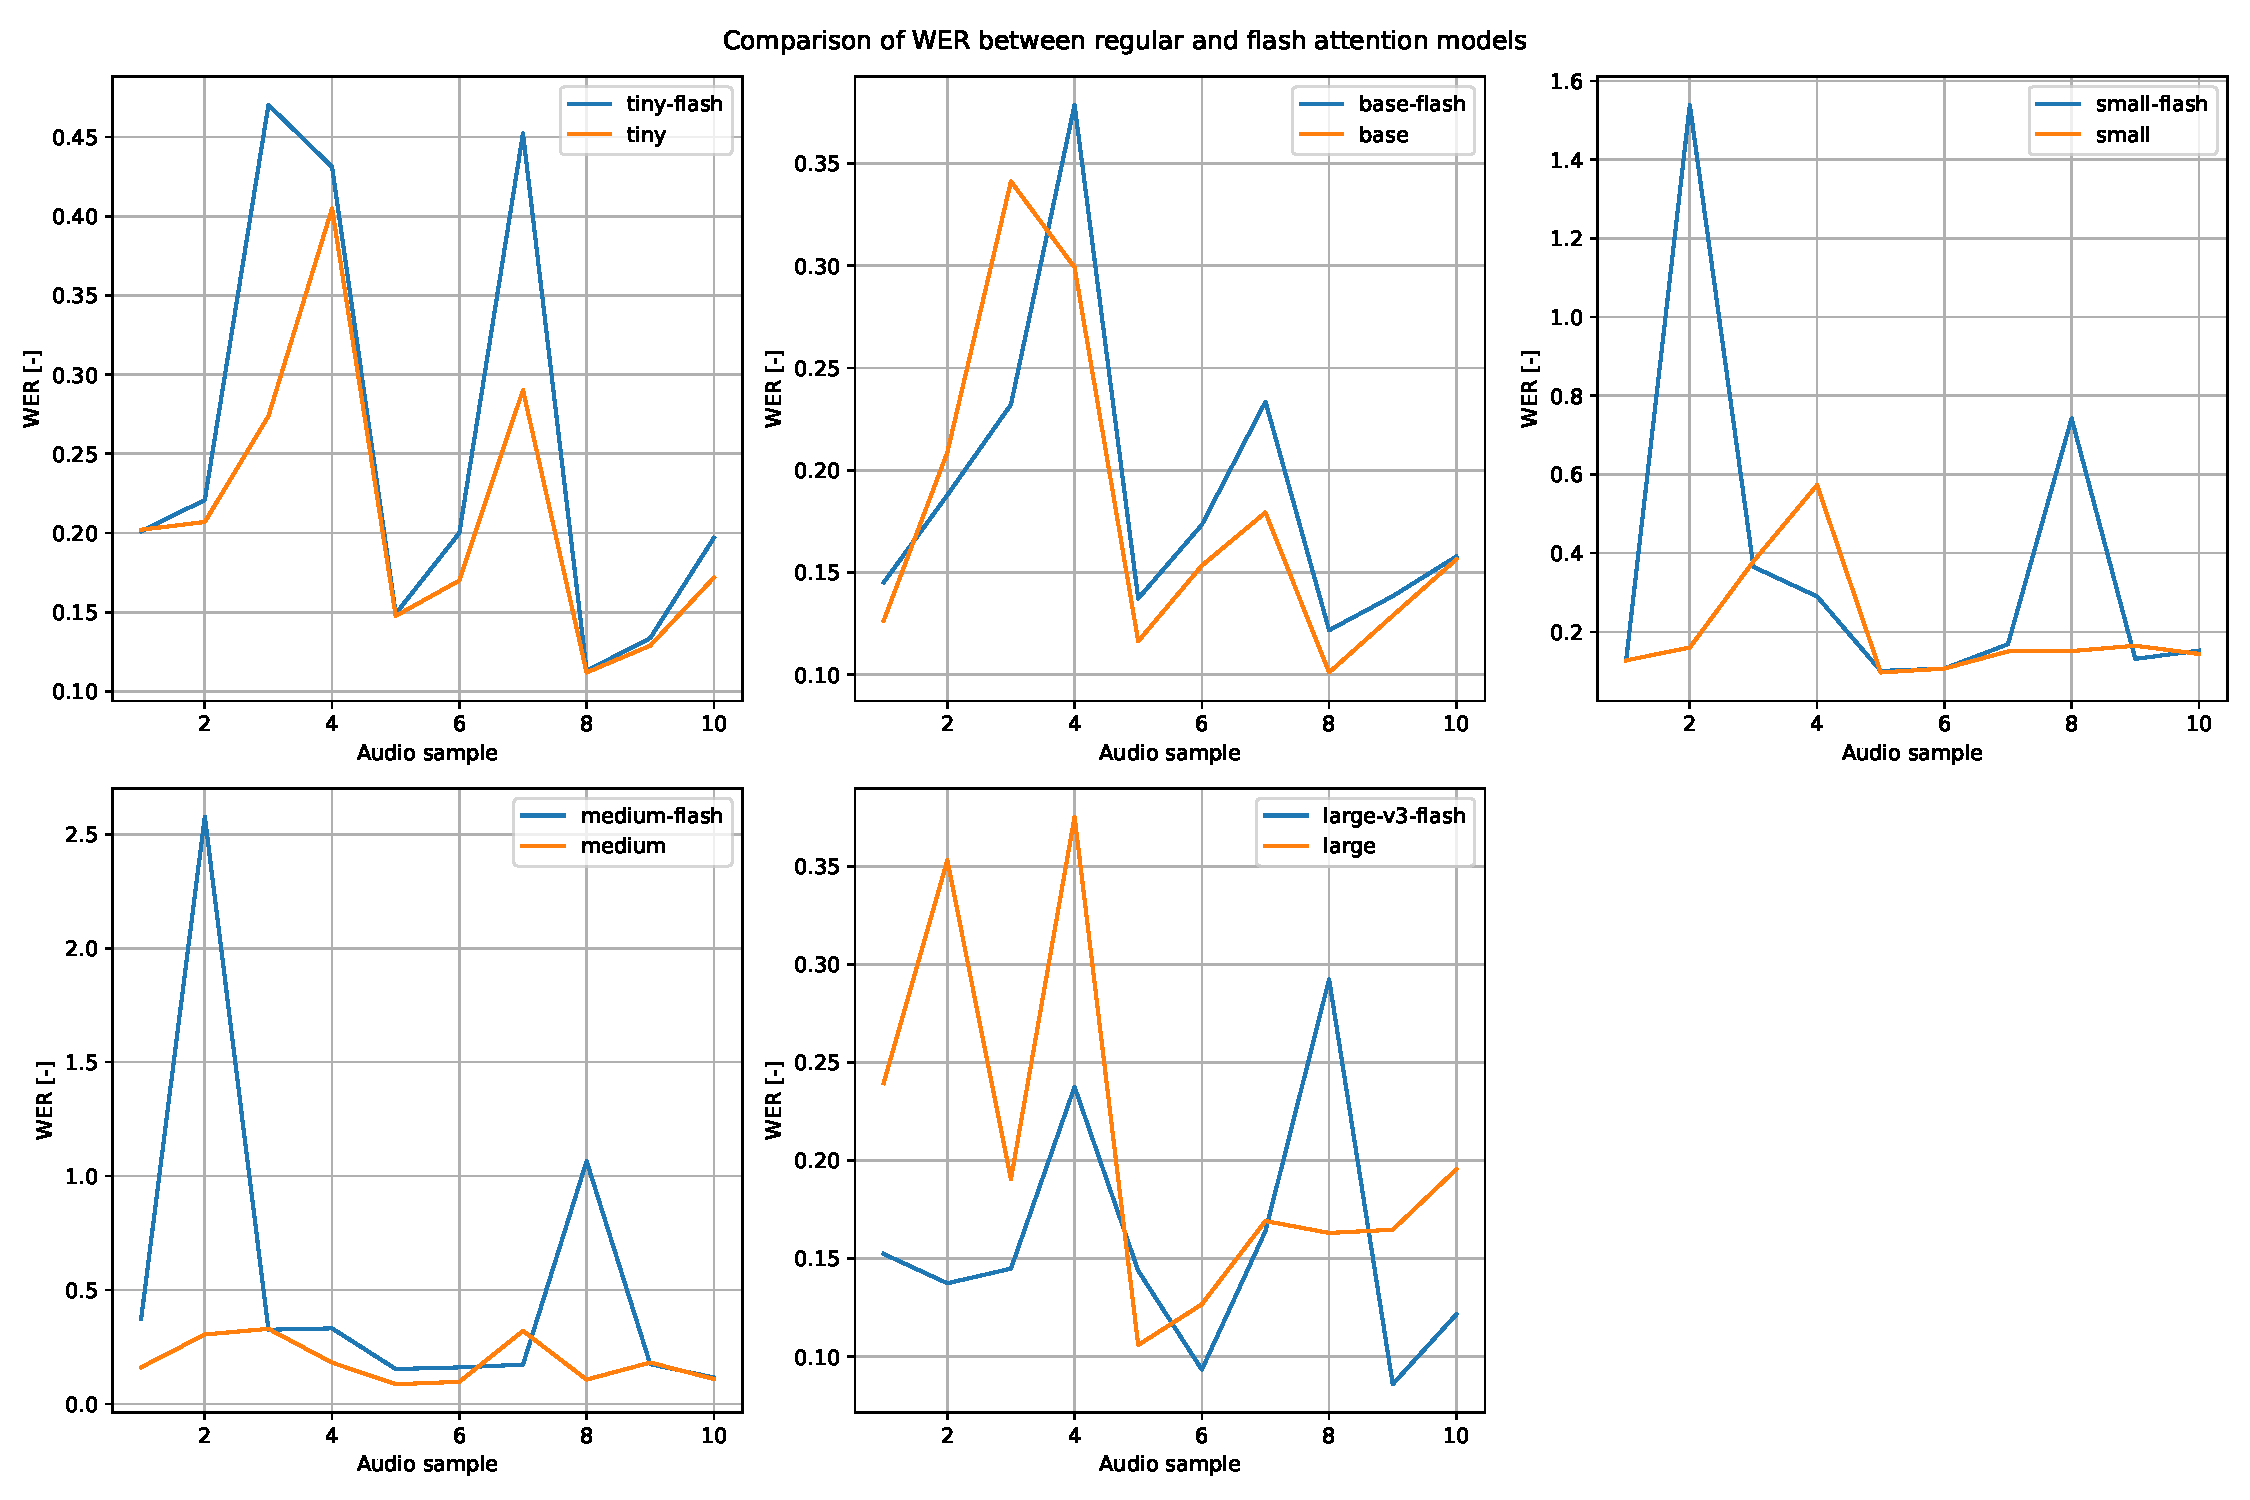
\includegraphics[width=\textwidth]{figures/wer.pdf}
    \caption{Caption}
    \label{fig:whisper_wer}
\end{figure}

\begin{figure}
    \centering
    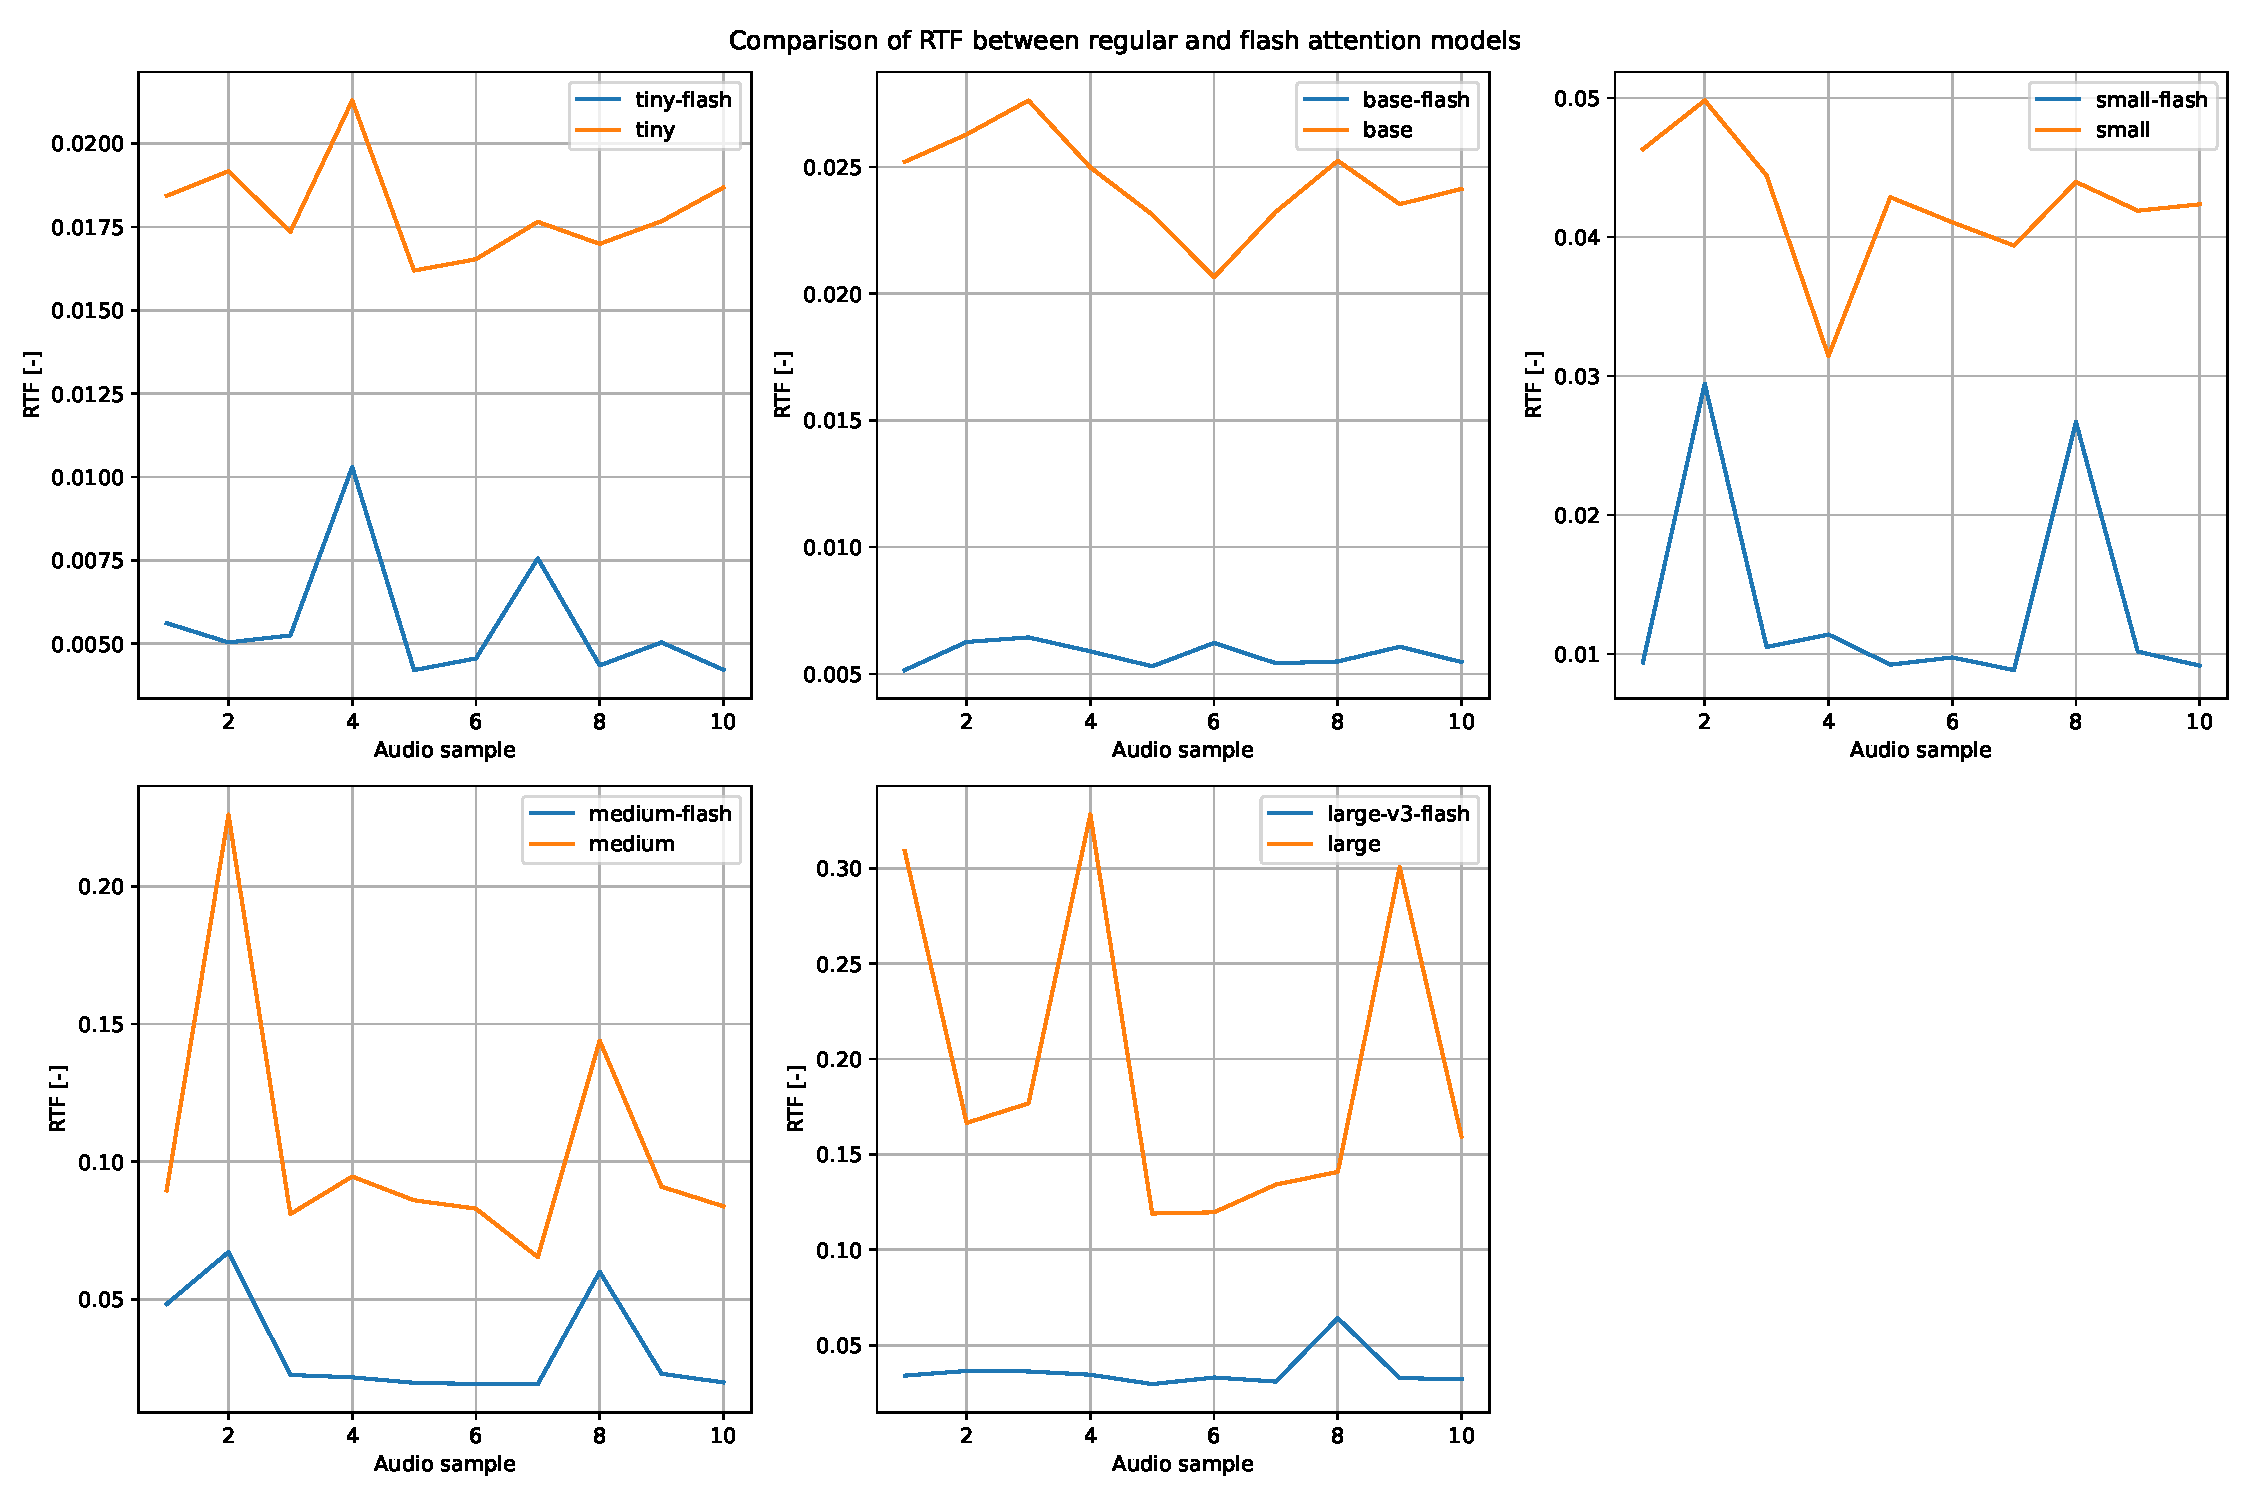
\includegraphics[width=\textwidth]{figures/rtf.pdf}
    \caption{Caption}
    \label{fig:whisper_rtf}
\end{figure}

\begin{figure}
    \centering
    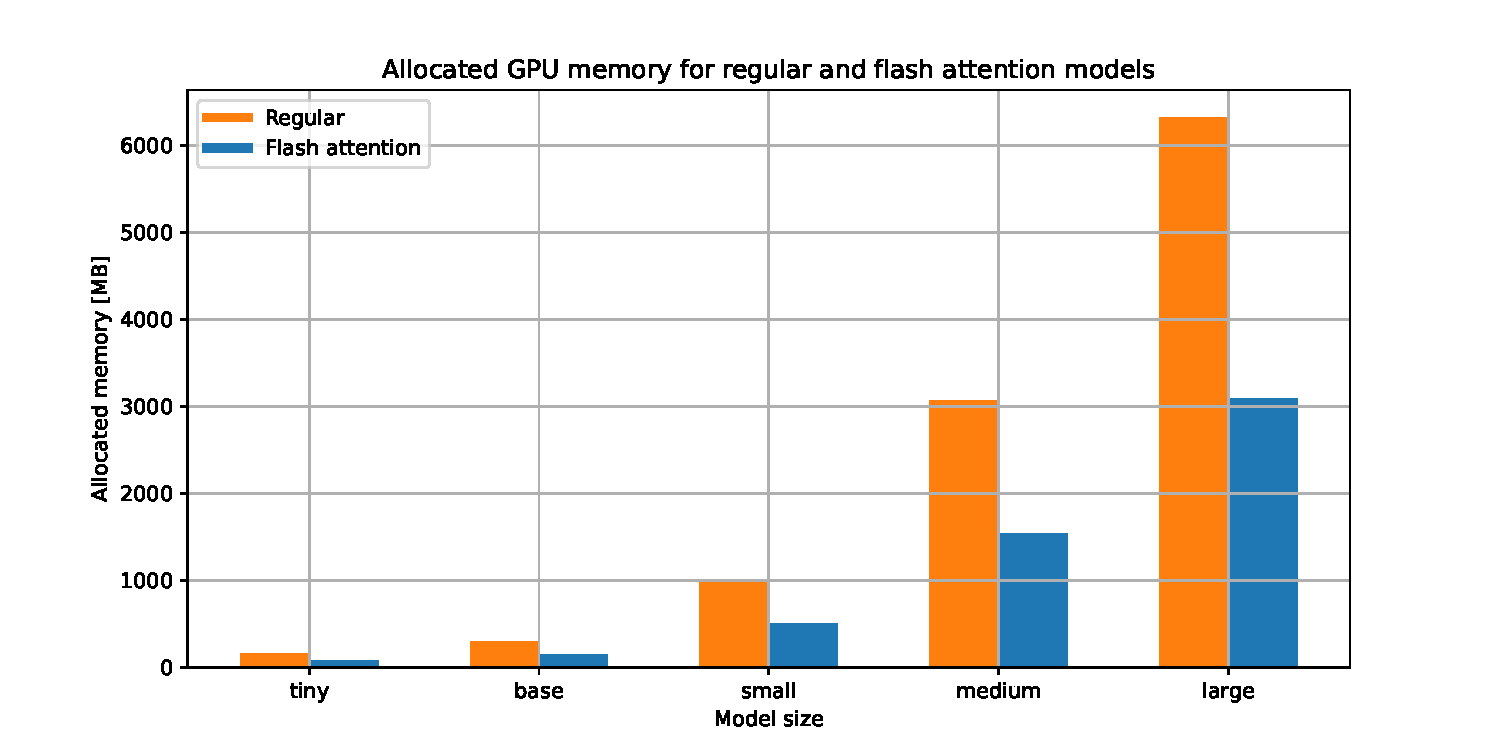
\includegraphics[width=\textwidth]{figures/memory.pdf}
    \caption{Caption}
    \label{fig:whisper_memory}
\end{figure}

\begin{figure}
    \centering
    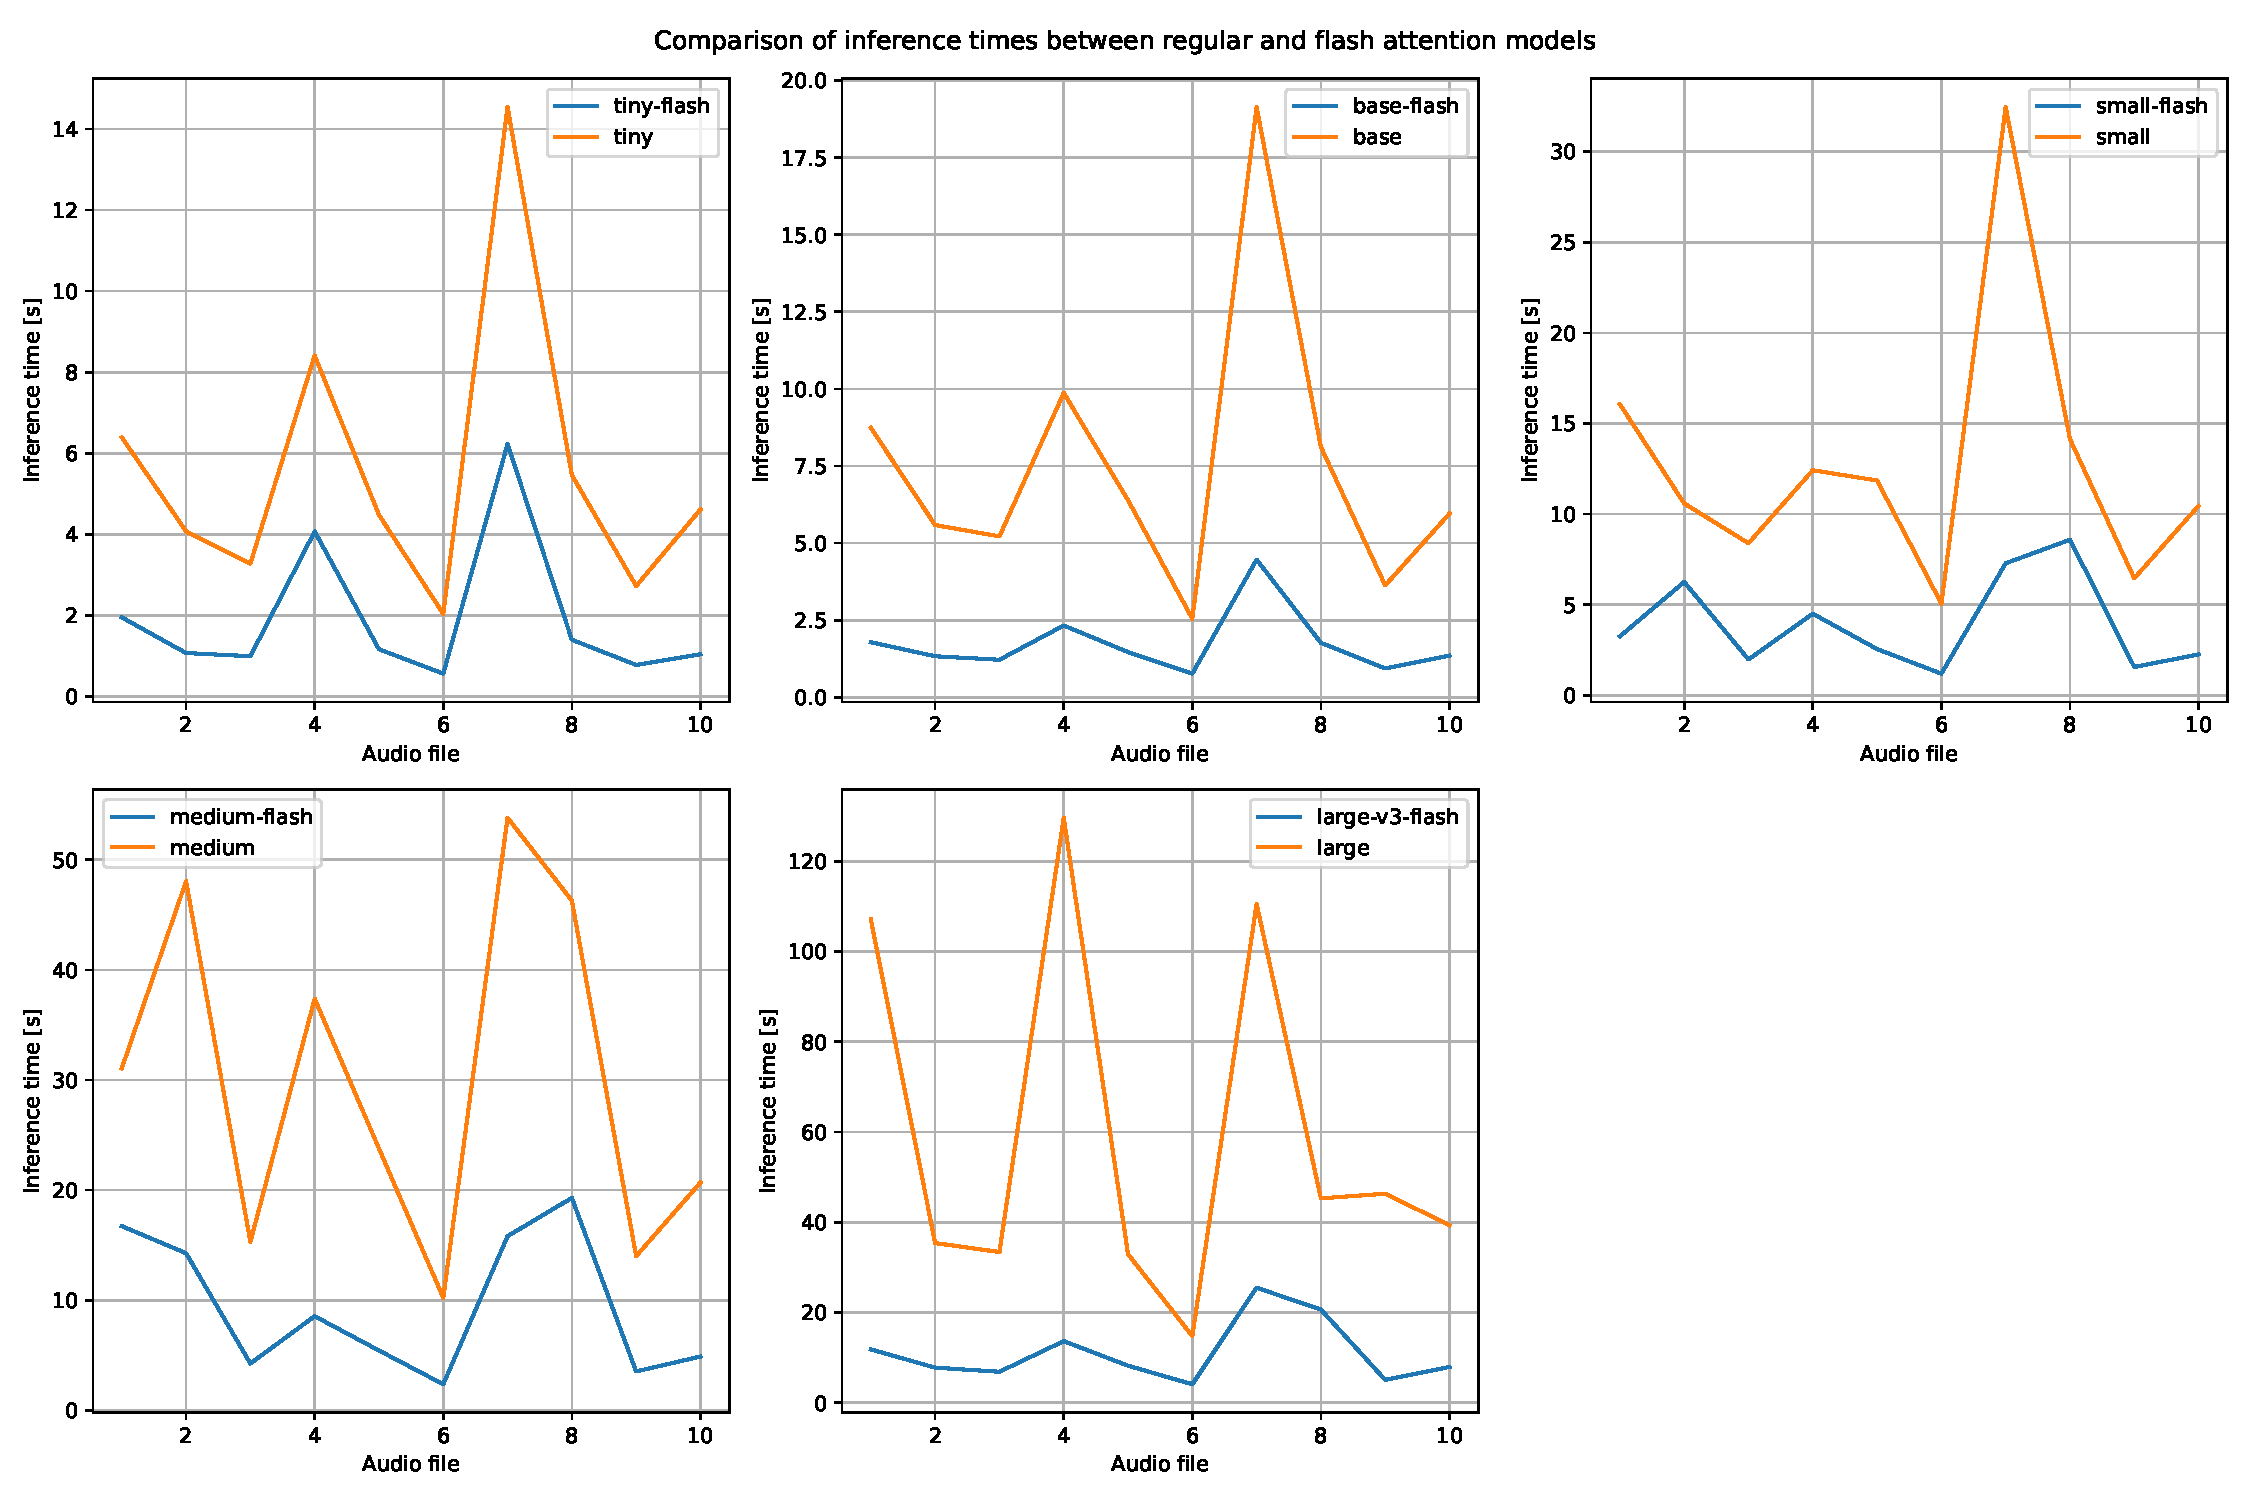
\includegraphics[width=\textwidth]{figures/inf_time.pdf}
    \caption{Caption}
    \label{fig:whisper_inf_time}
\end{figure}

\begin{figure}
    \centering
    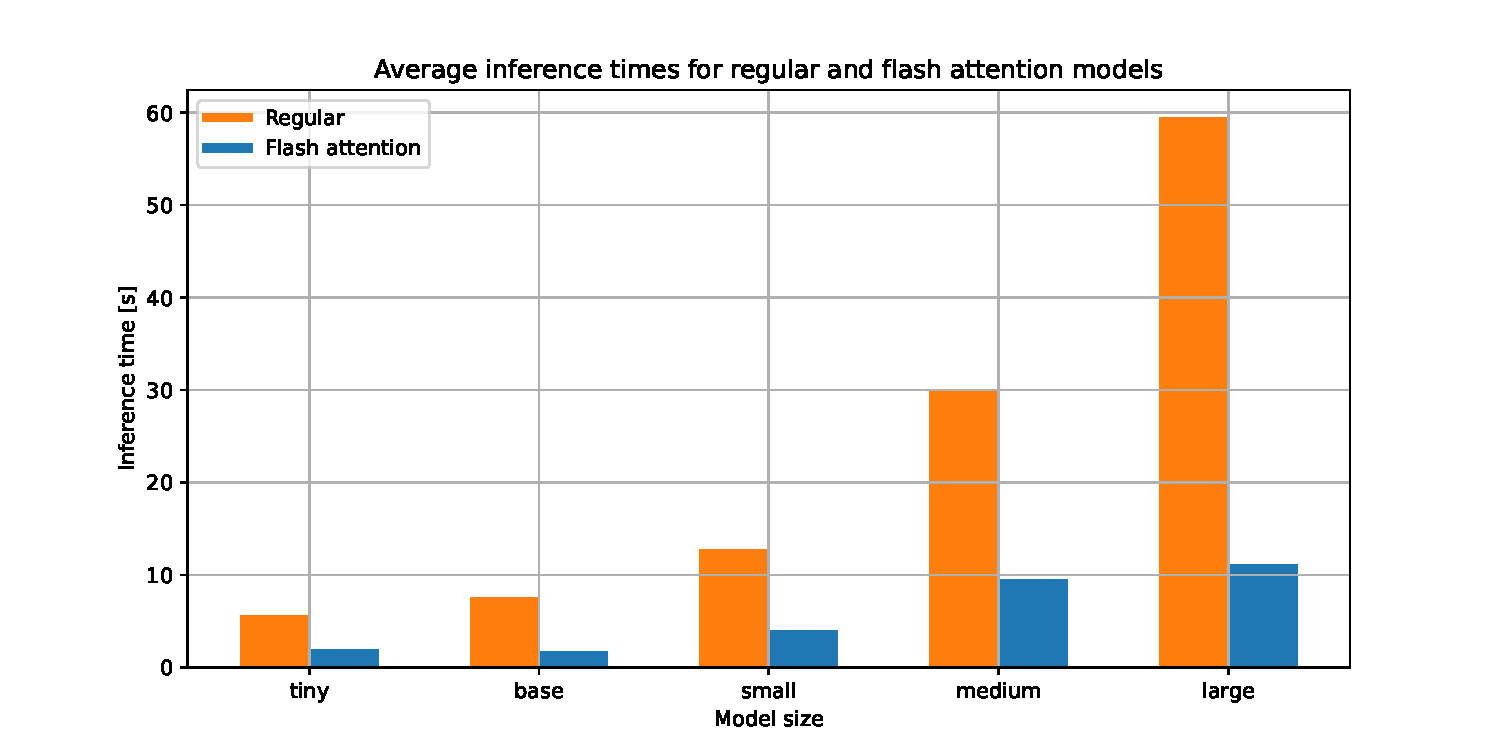
\includegraphics[width=\textwidth]{figures/avg_inf_time.pdf}
    \caption{Caption}
    \label{fig:whisper_avg_inf_time}
\end{figure}

\section{Mistral experiments}

\subsubsection{Example test set}

\begin{table}[]
\centering

\resizebox{\textwidth}{!}{%
\begin{tabular}{|l|l|l|}
\hline
\textbf{Domain}                                                                                                                                                                                                                                & \textbf{Command}                                                                                                                                                & \textbf{Solution}                                                                                                                                                                                                                                                                                                                                   \\ \hline
\begin{tabular}[c]{@{}l@{}}(:types worker task location)\\ \\ (:predicates\\ \\ (available ?worker - worker)\\ (assigned ?task - task ?worker - worker)\\ (located ?task - task ?location - location)\\ (completed ?task - task))\end{tabular} & \begin{tabular}[c]{@{}l@{}}Assign the new tasks to workers\\ efficiently. Task1 is at Location1,\\ Task2 at Location2.\\ Worker1 starts available.\end{tabular} & \begin{tabular}[c]{@{}l@{}}instance worker1 worker|\\ instance task1 task|\\ instance task2 task|\\ instance location1 location|\\ instance location2 location|\\ predicate available worker1|\\ predicate located task1 location1|\\ predicate located task2 location2|\\ goal assigned task1 worker1|\\ goal assigned task2 worker1|\end{tabular} \\ \hline
\end{tabular}%
}
\caption{One element of test set 1 with the domain and command given to Mistral, and a solution to compare the result.}
\label{tab:test_set}
\end{table}

\subsubsection{Example shot set}

\begin{table}[]
\centering
\resizebox{\textwidth}{!}{%
\begin{tabular}{|l|l|l|l|}
\hline
\textbf{Domain}                                                                                                                                                          & \textbf{Input}                                                                                                                                                                                                                                                                                                                                                                                    & \textbf{Output}                                                                                                                                                                                                                                                                                                                                                                                                                                                                                                  & \textbf{Label} \\ \hline
\begin{tabular}[c]{@{}l@{}}(:types portable location)\\ \\ (:predicates\\ \\ (at ?y - portable ?x - location)\\ (in ?x - portable)\\ (is-at ?x - location))\end{tabular} & \begin{tabular}[c]{@{}l@{}}Transport all the four objects to their\\ respective location: first object to\\ location 3, second object to location 0,\\ third object to location 1 and fourth\\ object at location 2. Also, go to location\\ 1 afterwards. The four objects are now\\ \\ at location 3, location 1, location 2 and\\ location 0 respectively. We are in\\ location 4.\end{tabular} & \begin{tabular}[c]{@{}l@{}}Here are the instances, predicates and goals:\\ instance l0 location|\\ instance l1 location|\\ instance l2 location|\\ instance l3 location|\\ instance l4 location|\\ instance o0 portable|\\ instance o1 portable|\\ instance o2 portable|\\ instance o3 portable|\\ predicate at o0 l3|\\ predicate at o1 l1|\\ predicate at o2 l2|\\ predicate at o3 l0|\\ predicate is-at l4|\\ goal at o0 l3|\\ goal at o1 l0|\\ goal at o2 l1|\\ goal at o3 l2\\ |goal is-at l1|\end{tabular} & Wrong          \\ \hline
\end{tabular}%
}
\caption{One element of shot set 2 labelled "Wrong". It is labelled "Wrong" due to the extra text in the output before the listing if instances.}
\label{tab:labeled_shot_set}
\end{table}

\subsubsection{Example system prompt}

\begin{table}[]
\centering
\resizebox{\textwidth}{!}{%
\begin{tabular}{|lll|}
\hline
\multicolumn{3}{|c|}{\textbf{Chat history}}                                                                                                                                                                                                                                                                                                                                                                                                                                                                                                                            \\ \hline
\multicolumn{1}{|l|}{System prompt}                                                                                                                                                                                                                                 & \multicolumn{1}{l|}{User content}                                                                                                                                                                     & Assistant content                                                                        \\ \hline
\multicolumn{1}{|l|}{\begin{tabular}[c]{@{}l@{}}As a PDDL assistant, your task is to\\ outline the available instances,\\ predicates, and goals based on the\\ provided domain and command.\\ Answer in the format shown after\\ \#\#\# Output \#\#\#\end{tabular}} & \multicolumn{1}{l|}{\begin{tabular}[c]{@{}l@{}}system\_prompt + f' Here is\\ a domain: \{domains{[}0{]}\},\\ and command \{inputs{[}0{]}\}.\\ \#\#\# Output \#\#\# \{outputs{[}0{]}\}.'\end{tabular}} & \begin{tabular}[c]{@{}l@{}}'Understood. Awaiting new\\ domain and command.'\end{tabular} \\ \hline
\end{tabular}%
}
\caption{Mistral's chat history with a system prompt before inference. The table must be read with a Python syntax from left to right.}
\label{tab:system_prompt}
\end{table}

\subsubsection{Generated knowledge}

\begin{table}[]
    \centering
    \resizebox{\textwidth}{!}{
    \begin{tabular}{|l|l|l|}
        \hline
        \textbf{Instances}     & \textbf{Predicates}                  & \textbf{Goals}    \\ \hline
        tars robot             & robot\_available tars                & \multirow{7}{*}{} \\ \cline{1-2}
        charging\_station zone & is\_recharge\_zone charging\_station &                   \\ \cline{1-2}
        unload\_zone zone      & is\_unload\_zone unload\_zone        &                   \\ \cline{1-2}
        shelf\_1 zone          & is\_shelf\_zone shelf\_1             &                   \\ \cline{1-2}
        shelf\_2 zone          & is\_shelf\_zone shelf\_2             &                   \\ \cline{1-2}
        shelf\_3 zone          & is\_shelf\_zone shelf\_3             &                   \\ \cline{1-2}
        shelf\_4 zone          & is\_shelf\_zone shelf\_4             &                   \\ \hline
        \end{tabular}
    }
    \caption{Instances and predicates that is true from the beginning of all specific PDDL domain tests. Notice that no goal is true from the beginning.}
    \label{tab:generated_knowledge}
\end{table}